\section{Grundlagen}
\subsection{Magnetooptischer Kerr-Effekt}
Der magneto-optische Kerr-Effekt (MOKE) beschreibt den Einfluss magnetischer Momente bei der Reflexion von Licht.
Er manifestiert sich in einer Drehung/"Anderung der Polarisation und Intensit"at des reflektierten Lichts.
Man unterscheidet prinzipiell zwischen drei Arten des MOKE, polarer, longitudinaler und transversaler MOKE.
Diese sind in Abbildung \ref{fig:moke_arten} gezeigt.
\begin{figure}[htpb]
    \centering
    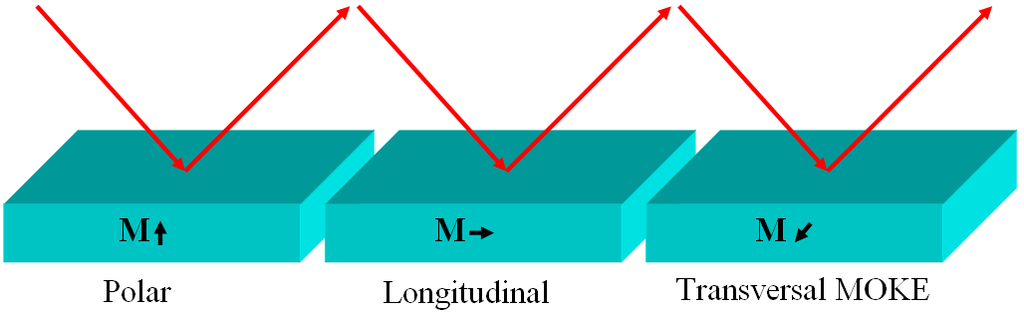
\includegraphics[width=0.8\textwidth]{../images/moke_arten.png}
    \caption{
        Die drei MOKE Arten: polar, longitudinal und transversal.
        Der Pfeil beschreibt die Richtung der magnetischen Polarisierung $M$ des Materials.
        Der blaue Pfeil zeigt Einfall und Reflexion des Lichts.\\
        Bild von: \url{https://upload.wikimedia.org/wikipedia/commons/thumb/b/b2/MOKE.PNG/1024px-MOKE.PNG}
        }
        \label{fig:moke_arten}
\end{figure}

F"ur die Anwendung bei optischen Speichermedien ist der polare MOKE (PMOKE) interessant.
Bei diesem ist die Magnetisierung senkrecht zur Oberfl"ache.
Bei diesem Effekt wird linear polarisiertes in elliptisch polarisiertes Licht umgewandelt und die Hauptachse wird um einen Winkel $\theta$ gedreht.
Erzeugt wird diese Drehung durch den sogenannten magnetisch zirkularen Dichroismus des Materials nach der Magnetisierung.
Dies bedeutet, dass es f"ur links und rechts zirkular polarisiertes Licht einen anderen Brechungsindex und Absorptionskoeffizienten hat.
Die beiden zirkularen Polarisationen erhalten daher eine andere Phasendifferenz und eine unterschiedliche Amplitude nach der Reflexion.
%TODO iclude a graphic
\cite{wikikerr}

\subsection{Optische Speichermedien}
\begin{figure}[htpb]
    \begin{minipage}[t][][t]{0.48\textwidth}
        \begin{tikzpicture}
        [x=0.07\textwidth, y=0.07\textwidth]
        \draw[color=blue, fill=blue]
            (0,-0.5) rectangle (10,0.5)
            (10.5,-0.5) node[right]{Lack};
        \draw[color=brown, fill=brown]
            (0,1) rectangle (10,3)
            (10.5,2.5) node[right]{Polyc}
            (10.5,1.5) node[right]{-arbonat};
        \draw[color=green, fill=green, opacity=0.7]
            (4.5,1) rectangle (6.5,5);
        \draw[color=green, fill=green]
            (10.5,4.5) node[right]{Laser};
        \draw[color=grey, fill=grey]
            (0,0)--(0,1)--
            (1,1)--(1,1.5)--(3,1.5)--(3,1)--
            (5,1)--(5,1.5)--(6,1.5)--(6,1)--
            (8,1)--(8,1.5)--(9,1.5)--(9,1)--
            (10,1)--(10,0)--
            (8.8,0)--(8.8,0.5)--(8.2,0.5)--(8.2,0)--
            (5.8,0)--(5.8,0.5)--(5.2,0.5)--(5.2,0)--
            (2.8,0)--(2.8,0.5)--(1.2,0.5)--(1.2,0)--
            (0,0)
            (10.5,0.5) node[right]{Al};
        \draw[color=black, <->]
            (5.5,5)--(5.5,1.5);
        \draw[color=red, <->]
            (6.25,5)--(6.25,1);
        \end{tikzpicture}
        \caption{
            Schematische Zeichnung einer CD.
            Die reflektierende Aluminium Oberfl"ache enth"alt kleine Buckel (\SI{0.38}{\micro\metre} breit).
            Gesch"utzt wird sie durch eine Lackschicht und eine Polycarbonat-Schicht.
            Der Laser erfasst ein Gebiet welches gr"o{\ss}er ist, als der Buckel.
        }
        \label{fig:CD}
    \end{minipage}
    \hfill
    \begin{minipage}[t][][t]{0.48\textwidth}
        \begin{tikzpicture}
        [x=0.1\textwidth, y=0.1\textwidth]
        \draw[color=brown, fill=brown]
            (0,1) rectangle (7,2.5)
            (7.5,1.5) node[right]{Substrat};
        \draw[fill=grey]
            (0,0) rectangle (3,1)
            (4,0) rectangle (5,1)
            (6,0) rectangle (7,1);
        \draw[fill=brightgrey]
            (3,0) rectangle (4,1)
            (5,0) rectangle (6,1);
        \draw[]
            (7.5,0.5) node[right]{MO-Schicht};
        \foreach \i in {0.25,0.75,1.25,1.75,2.25,2.75,4.25,4.75,6.25,6.75} {
            \draw[fill=black, shift={(\i,0.5)}, opacity=0.8]
                (-0.1,-0.4)--(-0.1,0.2)--(-0.2,0.2)--(0,0.4)--(0.2,0.2)--(0.1,0.2)--(0.1,-0.4)--(-0.1,-0.4);
        }
        \foreach \i in {3.25,3.75,5.25,5.75} {
            \draw[fill=black, shift={(\i,0.5)}, opacity=0.8]
            (-0.1,0.4)--(-0.1,-0.2)--(-0.2,-0.2)--(0,-0.4)--(0.2,-0.2)--(0.1,-0.2)--(0.1,0.4)--(-0.1,0.4);
        }
        \draw[color=green, fill=green, opacity=0.5]
            (3,0) rectangle (4,4);
        \draw[color=green]
            (7.5,3.5) node[right]{Laser};
        \end{tikzpicture}
        \caption{
            Magneto Optical device (MO).
            Die Information ist in der MO-Schicht in Form von Spins gespeichert.
            Durch den Kerr-Effekt wird die Polarisation des reflektierten Lasers um den Winkel $\theta$ gedreht.
        }
        \label{fig:MO}
    \end{minipage}
\end{figure}
In optischen Speichermedien sind die Informationen auf einem Datentr"ager gespeichert, von dem sie mit Hilfe eines Lasers ausgelesen werden.

Ein Beispiel ist die CD oder CD-ROM, wo die Information bin"ar in Form von kleinen Buckeln auf einer reflektierenden Oberfl"ache gespeichert wird.
Ein Laser (Wellenl"ange $\lambda=\SI{780}{\nano\metre}$) rastert die Oberfl"ache der CD ab.
Wie in Abbildung \vref{fig:CD} gezeigt, trifft er dabei eine Fl"ache, die gr"o{\ss}er ist, als ein Buckel.
Trifft er nur auf Land (das ist der Bereich wo kein Buckel ist) so haben alle reflektierten Strahlen die gleiche Phase.
Trifft er aber auf einen Buckel, so legt der Laserstrahl eine k"urzere Strecke zur"uck.
Diese ist so gestaltet, das die Phasendifferenz zwischen schwarzem und rotem Lichtweg $\lambda/2$ betr"agt.
Durch destruktive Interferenz wird die reflektierte Intensit"at verringert. \cite{wikicd}

Eine weitere Form von optischen Speichermedien sind Magnetooptische Discs (MO).
Bei diesen wird die Information, wie in Abbildung \vref{fig:MO} dargestellt, in der lokalen Magnetisierung gespeichert.
\cite{roll}


